\documentclass[10pt]{article}
\usepackage[margin=1in]{geometry}
\usepackage{cite}
\usepackage{amsmath}
\usepackage{amsfonts}
\usepackage{url}
\usepackage{graphicx}
\usepackage{multicol}

\title{MAUL: Machine Agent User Learning\footnote{Some unscrambling necessary.}\\ CS229 Project Report }
\author{Robert Holley and Daniel Rosenfeld}
\date{11/12/2010} 


\begin{document}
\maketitle
\begin{abstract}
We describe implementation of a classifier for User-Agent strings using Support Vector Machines.  The best Kernel is found to be the linear kernel, even when more complicated string based kernels, such as the edit distance kernel and the subsequence kernel, are employed.  A robust tokenization scheme is employed which dramatically speeds up the calculation for the edit string and subsequence kernels by shortening the effective string length. 
\end{abstract}
\begin{multicols}{2}

\section{Introduction}
A User-Agent string is an HTTP header sent along with a request for a web page, often but not always by a web browser.\cite{httprfc} The intent is to inform the server
of the capabilities of the software being used by the client. The User-Agent is
one of the most important signals to differentiate a desktop browser from a
mobile device or an automatic crawl. In addition gathering statistics on them
provides insights on changes in browser, operating system and device usage. They
are also frequently misused, in e.g. cloaking a web site to make it look
different to a search engine crawl.

User-Agent strings can contain loosely-structured tokens on engine, browser,
version, build date, etc. but their format was never strictly standardized.\cite{httprfc}
As the number of web-access devices increases, especially with new-generation
mobile devices and browsers, the numbers of different User-Agent strings is
rapidly growing and diversifying. Extensions and plugins can often mutate
User-Agent strings in unpredictable ways (insert, splitting, duplicating, and
re-ordering tokens). Firefox 4 and Internet Explorer 9 will soon ship with
completely reformatted strings. Some mobile operators have begun introducing
custom HTTP headers to extend the traditional role of the User-Agent.\cite{mobile} Web spiders and crawlers are also an important and unpredictable contributing factor.
An overview of the development and mutation of User-Agent strings is given in,\cite{history} while \cite{uatracker} is a public list of over 50000 currently unique strings.

For over a decade, those interested in tracking the proliferation of the web have collected User-Agent strings and built classifiers for them.  One of the first such entities was Microsoft, who included a recognition engine (browscap.dll) and a pattern file (browscap.ini) with its early web servers.\cite{bcp}  The Browser Capabilities Project (BCP) has kept these files up to date for the web development community, despite Microsoft's abandonment for more sophisticated (and proprietary) methods.\cite{bcp}  However, the maintenance of the project requires human parsing of new User-Agent strings every week and subsequent updating of the recognition engine and pattern file (BCP reports that they receive several dozen new User-Agent strings per week).  Gary Keith, the proprietor of BCP, has an automatic script run every Sunday morning, the output of which he parses in the afternoon and subsequently updates his file of highly structured regular expression searches.  A more recent effort, Browserscope (which started as UAProfiler), took a similar approach, using a regular expression based parsing engine to identify specific browsers (browsers only). \cite{souders}  The parsing engine required regular updates to remain up to date with new User-Agent strings.  In 2009, the author of UAProfiler (Steve Souders) reported finding 20 new User-Agent strings {\it per day}, which he examined every day at 7 am over morning coffee. \cite{souders2}  Other efforts such as those by user-agent-string.info and useragentstring.com, also use brittle parsing rules and curated data just like Browserscope and BCP.  \cite{uas.info,uas.com}  Other efforts to categorize User-Agent strings include entire communities such as agentarius.net, which has created a structured database of over 200,000 User-Agent strings.   

Our machine learning approach to User-Agent string parsing could provide partially automated parsing even on new User-Agent strings, absolving the need for a human to keep User-Agent parsers up to date.  Although we are quite sure Gary and Steve will continue updating their parsers each Sunday and over morning coffee, perhaps some day in the future this will not be necessary.

\section{Computational Approach}
\subsection{Data}
We have assembled an annotated dataset consisting of 53,829 User-Agent strings.  The strings were acquired from a variety of sources (user-agents.org: 2463 strings, ua-tracker.com: 50,482 strings, user-agent-string.info: 1460 strings; 53,829 total excluding duplicates.).\cite{ua.org,uatracker,uas.info}  The annotation consists of agent type (Browser, Bot), agent family (Firefox, googlebot, etc.), family version, OS (Windows, Linux, etc.), and OS version.  The annotation was performed by using two common parsing engines (UASparser\cite{uas.info} and uaParser (formerly Browserscope, formerly UA Profiler)\cite{uaParser} )) and merging the result.  Since UASparser returns the most information (a Python dictionary with User-Agent Type, Family, and OS) it is used as the primary source of information whereas uaParser is used to generate version information for Browsers.  uaParser is primarily geared toward parsing Browsers and therefore is not useful for Bots and the other types of entities on the web.   This approach was taken due to the lack of availability of annotated sources.  Some of the annotated User-Agent strings were curated by hand due to the failure of the parsers.  The data were parsed and annotated using a series of python scripts and python versions of the afore-mentioned parsers.  
\subsection{Data Processing}
The data generated by the above methods were additionally processed to reduce and standardize the number of classes.  Specifically, the OS information was parsed to collapse all versions of Windows, Linux and Mac OS into only three OS's and move all other OS information into the OS version field.  All special versions/modes/builds of specific Browsers were collapsed into their respective families.  All Validators and Bots were given the Type field ``Robot" since Validators are also non-human web crawler applications.  The dataset is stored in both a flatfile format which allows for facile reading and editing by a human and a SQLlite database for use by classifier codes.  
%tokenization in this section, and data pipeline
% - some testing of tokenization, i.e. addition of @, + , &
% tokenization figure
The User-Agent strings were tokenized in order to build feature vectors and also speed up the implementation of the non-vector based string Kernels we used to classify the strings.  Tokenization is an atomistic deconstruction of each User-Agent string at arbitrarily chosen break characters (See Figure 1).  The tokenization scheme used in our classifiers was to break apart the string at any instance of {\bf \textbackslash / [].,;}.  Other break characters were also attempted, such as `@' and `\&', however little improvement resulted.  

The tokens were further coalesced to increase the robustness of the classifier.  Instead of having a unique token for every number, all numbers of the same length were represented by a single token.  Further coalescing was performed so that instances of `http' and `+http' were represented by a single token.      

\begin{figure}
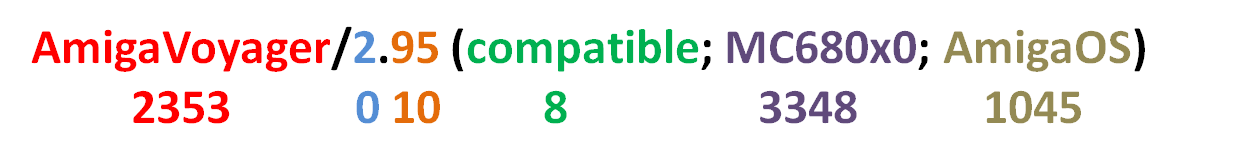
\includegraphics[width=3.5in]{token_figure.png}
\caption{Example of the tokenization process.  Notice that the string is de-constructed at any instance of one of the following characters: {\bf \textbackslash /[].,;}  .}
\end{figure}


\subsection{Learning}
% few sentences on SVM, overfitting protection
% figure on decision tree
Generally, given a new User-Agent string, our goal is to guess whether the string is from a bot, a browser or a mobile browser.  If the string is from a browser, we will also want to guess the browser type (family) and OS type.    Our goal is to build several classifiers using different techniques in order to find the most robust for classifying User-Agent strings.  For performing SVM training and prediction we use the LIBSVM-String library library (see implementation section below).\cite{libsvm}\cite{libsvm-string}  

The kernels we chose to test are the linear, radial basis function (Gaussian), edit string (tokenized), and subsequence (tokenized, see implementation below).  The edit string kernel is defined as
\begin{equation}
K(x,z) = \exp \left[ - \gamma \operatorname{LD}(x,z) \right]
\end{equation}
where $\operatorname{LD}$ is the Levenshtein edit distance between the strings $x$ and $z$.  As input parameters, the edit distance kernel takes the decay factor $\gamma$.  The subsequence kernel is calculated in a less straightforward manner.  This kernel seeks to compare all non-contiguous sub-strings of length $p$ between two strings.\cite{subseqkernel}  Given that the string is expressed in an alphabet of size $|\mathcal{A}|$, the feature vector $\phi(x) \in \mathbb{R}^{|\mathcal{A}|^p}$.  Each element in the feature vector corresponds to a possible sub-string, $u$, of length $p$ in alphabet $|\mathcal{A}|$.  The entry for each element is 
\begin{equation}\phi_u(x) = \sum_{i \in \text{instances}(u,x)} \lambda^{\operatorname{length}(i)}
\end{equation}
where the notation $ \text{instances}(u,x)$ means all instances of the sub-string $u$ in $x$.  The inner product between two vectors is then simply  the normal inner product between two feature feature vectors $\phi(x)$, $\phi(z)$.  Any sub-string which is not present in a string has a $0$ entry in the $u$ position of the feature vector, indicating that the inner product corresponds to a sum over all shared length $k$ sub-strings.  As inputs the subsequence kernel takes in a desired sub-string length $p$ and a decay factor $\lambda$.

All of our classifiers are of the multi-class variety.  Our multi-class classifiers are of the one-vs.-one, max-wins variety.  This means that for a problem of $k$ classes, we form $\frac{k(k-1)}{2}$ one-vs.-one classifiers.  For prediction on an input string, the input string is passed through all classifiers, and the class that was predicted most frequently is returned as the prediction.  

\section{Implementation}

In our efforts, we developed a  versatile software stack for classifying User-Agent strings. The code is open-source and available at \url{https://github.com/bholley/maul}. In this section, we briefly describe the key components.


\subsection{libsvm-string}

At the heart of our implementation is LIBSVM-string, a superset of libsvm that includes the ability to classify string data. \cite{libsvm-string} When invoked with the proper parameters, LIBSVM-string accepts arrays of characters (rather than vectors) as input data, and operates on them with a string kernel.

LIBSVM-string comes standard with an implementation of the edit distance kernel. For comparison, we also implemented a recursive subsequence kernel, basing our work on example code from \cite{learning-kernel-classifiers}. Unfortunately, the subsequence kernel turned out to be significantly slower than the edit kernel, with time spent in the kernel function dominating training and testing time. During profiling, we discovered that half of the total computational time was spent inside the \texttt{pow()} function computing various powers of $\lambda$ (the decay parameter). Since this parameter is constant for a given SVM, we restructured the code to make the subsequence kernel stateful. On the first call, the kernel precomputes all necessary powers of lambda, so that subsequent calls can retrieve the appropriate values from a look-up table.

This doubled the performance of our SVM, but training with a small fraction of our training data still took over an hour. We determined that the performance of the subsequence kernel was cubic in its input string. Thus, the most effective way to speed up the algorithm would be to reduce the size of the input. To do this, we introduced a tokenizer, which mapped ASCII strings to sequences of tokens (represented as 4-byte unsigned integers). This had the effect of dramatically increasing the alphabet size (from $2^8$ to $2^{32}$), while dramatically decreasing the average string length. We made the necessary generalizations in the data structures and control logic, and templatized the kernel function (replacing \texttt{char*} with \texttt{T*}), allowing us to use the exact same code for both data types.

One major problem with libsvm-string was that it didn't include a good memory ownership model for string data. In particular, it would assume that the data pointed to by a \texttt{char*} remained immutable between calls into the library, and would not make any internal copies of the training data. This assumption was not valid for our use cases, leading to crashes. We thus introduced a memory management system where we make copies of input data and track whether structures were allocated within LIBSVM or outside of it, allowing LIBSVM to clean up its own memory but avoid clobbering the memory of its caller.

\subsection{Python Framework}

Since we were operating primarily on string data, we decided that it would be unnecessarily painful to write all of our code in C or C++. We settled on Python as a harness language, and wrote a flexible and robust framework on top of LIBSVM-string using the CTypes module of Python. This turned out to be less straightforward than we had originally thought, and we eventually had to make a few small changes to LIBSVM-string to work around CTypes bugs on certain operating systems.

In the end, it turned out to be worth it. Using our MAUL framework, any cross-validation procedure with any set of parameters can be implemented with only a few lines of code (see \texttt{MaulHarness.py} and \texttt{MaulBatch.py}). The framework includes automatic model saving, data selection, and built-in validation. The data was managed with an SQLite database, so that training and testing data could be selected quickly and efficiently from our highly heterogeneous data sources. Finally, it allows string and vector SVMs to be instantiated and used with the same code. As a result, the finished framework made it extremely easy to compile our final results. We wrote a small python program to repeatedly call the cross-validation routine with different sets of parameters, and let it run overnight.

% Results
% - Kernel competition
%  	- results table
% - cases where classification can beat traditional parsing
% - ordering as a confounding factor
% - cross validation for parameter tuning
% -  
\section{Results and Discussion}
Classifiers using the afore-mentioned kernels were built to determine whether a User-Agent string is a Browser/Robot/Mobile Browser (B/MB/R), which family (IE, Chrome, Firefox, etc.) a Brower belongs to (Fam.), and which OS a Browser type User-Agent string reports (OS).  The below table summarizes the accuracy results for the given classifiers.  These classifiers were run using the parameters ($C = 1.0$, $\gamma = 0.1$, $p = 5$, $\lambda = 0.8$)
\begin{center}
\begin{tabular} { r | r | r | r}
Kernel\textbackslash Accuracy(\%) & B/MB/R & Fam. & OS \\
\hline
Linear & 99.68 & 99.81 & 99.90 \\
RBF & 99.51 & 98.69 & 99.66 \\
Edit String & 99.60 & 98.61 & 99.68 \\
Subsequence & 99.30 & 99.28 & 99.67 \\
\end{tabular}
\end{center}

The above table demonstrates that the linear classifier, despite its simplicity, performs better than all other kernels.  This is surprising given the more complicated feature space implied by some of the other kernels.  For example, both edit string and subsequence kernels include information regarding the ordering and position of tokens within a string.  Our results suggest that this information is of little use in classifying User-Agent strings.  Possible reasons include the shuffling of tokens in User-Agent strings due to browser plugins, browser build differences, or other mechanisms.  In Robot vs. Other classification, the Robot strings are typically short and in a more standard format, suggesting perhaps ordering information is not necessary for good classifiers.  

The data was further inspected post-hoc to determine whether our SVM based classifier was superior to regular expression based parsers.  Some types of strings are expected to be difficult to classify for standard parsers, specifically: robots never seen before, robots disguised as browsers, and browsers that are partially disguised as robots.  We have found an instance of each of these cases, where when the below strings are excluded from the data they are still classified properly, yet several online tools fail at classification.  The examples we found were: 

The robot with the User-Agent string, Mozilla/5.0 (compatible; Butterfly/1.0; \\+http://labs.topsy.com/butterfly/) Gecko/2009032608 Firefox/3.0.8, is a bot disguised as a browser, and was misclassified by uaProfiler, useragentstring.com, and user-agent-string.info. 
The robot with the User-Agent String,  ArabyBot (compatible; Mozilla/5.0; GoogleBot; FAST Crawler 6.4; http://www.araby.com;), is a bot that was not seen before, and went unclassified by uaProfiler, user-agent-string.info, useragentstring.com and Agentarius.  
The browser with the User-Agent string, Googlebot/2.1 (+http://www.googlebot.com/bot.html; MSIE 7.0; Windows NT 5.1; GoogleT5; .NET CLR 2.0.50727; .NET CLR 3.0.4506.2152; .NET CLR 3.5.30729; .NET CLR 1.1.4322), is a browser disguised as a bot, and was misclassified by user-agent-string.info and BCP (the more browser centric parsers uaProfiler and useragentstring.com did get this one right).  

For the type classifier (B/MB/R) some effort was expended in cross-validating the input kernel parameters.  However, little if any improvement was achieved.  Changing the parameters $\gamma$, $\lambda$, and $p$ did not result in any improvement in the performance of the edit and subsequence kernels relative to the linear kernel.  Changing the parameter C had some effect on the performance of the classifiers, although $C = 1.0$ was close to optimal and only improvement at the hundredth of a percent level was achieved for the linear classifier with $C = 3.0$.  This lack of improvement could be due to the ``ease" in classifying a User-Agent string, and testifies to the power of the SVM based classifier with respect to this data class.

\section{Extensions}

Our classification efforts were highly successful, but there is still much to be done. The Mozilla Corporation has expressed interest in using MAUL in its Metrics \& Analytics group, so we hope that work on this topic will continue. User-Agent classification is a rich and nuanced problem, and there are a number of interesting extensions that we did not have the resources to explore. We list a few of them here:

\subsection{Improved Cross-Validation and Tokenization}

We did some cursory testing to select our set of token delimiters, but it was far from a rigorous process. It would be interesting to use formal cross-validation and feature-selection techniques to select the optimal separators.

Also, our attempt to cross-validate the input kernel parameters could be improved by using k-fold cross-validation (instead of a held out test set).  

\subsection{Improved Token Coalescence}

The SVM treats all tokens as equally distinct, regardless of the true similarity between any two tokens. We implemented some manual coalescing of tokens. For example, we replaced any integer with its number of digits (ie, 14 and 36 are treated as the same number). Nonetheless, there are many other approaches worth exploring:

\begin{itemize}
\item Other common patterns (for example, email addresses)
\item Coalescing the most infrequent tokens into a single 'Other' token
\item Using one of the string kernels to identify the nearest neighbor to an infrequent token (this would allow for User-Agent strings with new tokens to be classified, despite having tokens in the classifier feature set)
\end{itemize}


\subsection{Larger Datasets}
Our training set was large, but not exhaustive. There are many other sources of User-Agent data on the web (including sites like Agentarius.net, as mentioned above), and we believe that the size of our dataset could increase by an order of magnitude with reasonable effort.

\section{Summary of Results}
A new class of text data has been successfully classified using SVM techniques and the results of using several kernels have been compared.  Little improvement is found over using the linear kernel.  A tokenization scheme is described that allows for large speed improvements in using string based kernels.  An easy to use Python based framework was developed that allows for rapid training and testing using a modified LIBSVM-String library.  

\end{multicols}


\bibliography{references}
\bibliographystyle{plain}
\end{document}
